\message{ !name(teoria.tex)}\documentclass[a4paper,12pt, oneside]{book}

% \usepackage{fullpage}
\usepackage[italian]{babel}
\usepackage[utf8]{inputenc}
\usepackage{amssymb}
\usepackage{amsthm}
\usepackage{graphics}
\usepackage{amsfonts}
\usepackage{listings}
\usepackage{amsmath}
\usepackage{amstext}
\usepackage{engrec}
\usepackage{rotating}
\usepackage{verbatim}
\usepackage[safe,extra]{tipa}
%\usepackage{showkeys}
\usepackage{multirow}
\usepackage{hyperref}
\usepackage{microtype}
\usepackage{fontspec}
\usepackage{enumerate}
\usepackage{physics}
\usepackage{braket}
\usepackage{marginnote}
\usepackage{pgfplots}
\usepackage{cancel}
\usepackage{polynom}
\usepackage{booktabs}
\usepackage{enumitem}
\usepackage{framed}
\usepackage{pdfpages}
\usepackage{pgfplots}
\usepackage{algorithm}
% \usepackage{algpseudocode}
\usepackage[cache=false]{minted}
\usepackage{mathtools}
\usepackage[noend]{algpseudocode}

\usepackage{tikz}\usetikzlibrary{er}\tikzset{multi  attribute /.style={attribute
    ,double  distance =1.5pt}}\tikzset{derived  attribute /.style={attribute
    ,dashed}}\tikzset{total /.style={double  distance =1.5pt}}\tikzset{every
  entity /.style={draw=orange , fill=orange!20}}\tikzset{every  attribute
  /.style={draw=MediumPurple1, fill=MediumPurple1!20}}\tikzset{every
  relationship /.style={draw=Chartreuse2,
    fill=Chartreuse2!20}}\newcommand{\key}[1]{\underline{#1}}
  \usetikzlibrary{arrows.meta}
  \usetikzlibrary{decorations.markings}
  \usetikzlibrary{arrows,shapes,backgrounds,petri}
\tikzset{
  place/.style={
        circle,
        thick,
        draw=black,
        minimum size=6mm,
    },
  transition/.style={
    rectangle,
    thick,
    fill=black,
    minimum width=8mm,
    inner ysep=2pt
  },
  transitionv/.style={
    rectangle,
    thick,
    fill=black,
    minimum height=8mm,
    inner xsep=2pt
    }
  } 
\usetikzlibrary{automata,positioning,chains,fit,shapes}
\usepackage{fancyhdr}
\pagestyle{fancy}
\fancyhead[LE,RO]{\slshape \rightmark}
\fancyhead[LO,RE]{\slshape \leftmark}
\fancyfoot[C]{\thepage}
\usepackage[usenames,dvipsnames]{pstricks}
\usepackage{epsfig}
\usepackage{pst-grad} % For gradients
\usepackage{pst-plot} % For axes
\usepackage[space]{grffile} % For spaces in paths
\usepackage{etoolbox} % For spaces in paths
\makeatletter % For spaces in paths
\patchcmd\Gread@eps{\@inputcheck#1 }{\@inputcheck"#1"\relax}{}{}
\makeatother

\title{Teoria dell'Informazione e Crittografia}
\author{UniShare\\\\Davide Cozzi\\\href{https://t.me/dlcgold}{@dlcgold}}
\date{}

\pgfplotsset{compat=1.13}
\begin{document}

\message{ !name(teoria.tex) !offset(-3) }

\maketitle

\definecolor{shadecolor}{gray}{0.80}
\setlist{leftmargin = 2cm}
\newtheorem{teorema}{Teorema}
\newtheorem{definizione}{Definizione}
\newtheorem{esempio}{Esempio}
\newtheorem{corollario}{Corollario}
\newtheorem{lemma}{Lemma}
\newtheorem{osservazione}{Osservazione}
\newtheorem{nota}{Nota}
\newtheorem{esercizio}{Esercizio}
\algdef{SE}[DOWHILE]{Do}{doWhile}{\algorithmicdo}[1]{\algorithmicwhile\ #1}
\tableofcontents
\renewcommand{\chaptermark}[1]{%
  \markboth{\chaptername
    \ \thechapter.\ #1}{}}
\renewcommand{\sectionmark}[1]{\markright{\thesection.\ #1}}
\newcommand{\floor}[1]{\lfloor #1 \rfloor}
\newcommand{\MYhref}[3][blue]{\href{#2}{\color{#1}{#3}}}%
\chapter{Introduzione}
\textbf{Questi appunti sono presi a lezione. Per quanto sia stata fatta
  una revisione è altamente probabile (praticamente certo) che possano
  contenere errori, sia di stampa che di vero e proprio contenuto. Per
  eventuali proposte di correzione effettuare una pull request. Link: }
\url{https://github.com/dlcgold/Appunti}.\\
\chapter{Introduzione}
Si ha una sorgente che emette messaggi e li vuole mandare tramite un canale di
comunicazione, che contiene del rumore che agisce sui messaggi e li rovina. Il
destinatario per capire che il messaggio è rovinato ha varie tecniche. Una
prima cosa che potrebbe fare è chiedere di rimandare il messaggio ma sarebbe
meglio correggere \textit{in loco} e si hanno algoritmi per farlo (tra cui lo
\textbf{schema di Hamming} usando il modello del \textbf{rumore bianco}).\\
Un'altra tematica è la codifica stessa del sorgente, comprimendo flussi di dati,
senza perdere informazioni.\\
Si parlerà anche dei canali di comunicazione, delle capacità e dei
\textbf{teoremi di Shannon}. \\
Si vedranno poi le basi della crittografia, i crittosistemi storici, vari
standard etc$\ldots$
\chapter{Teoria dell'informazione}
Si hanno due sottoparti principali:
\begin{itemize}
  \item \textbf{teoria dei codici}, per individuare e correggere gli errori. Si
  studia il canale di trasmissione cercando di contrastare il rumore che c'è nel
  canale
  \item \textbf{teoria dell'informazione}, in cui il focus è la sorgente delle
  informazioni
\end{itemize}
Vediamo il classico schemino della teoria dell'informazione:
\begin{figure}[H]
  \centering
  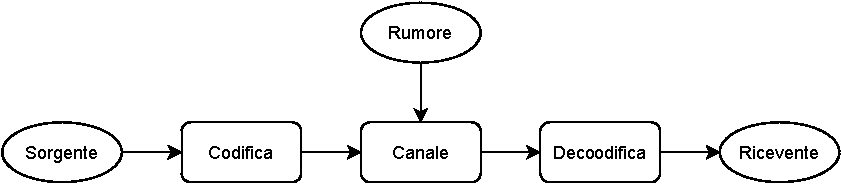
\includegraphics[width = \textwidth]{img/teo.pdf}
  \caption{Schema di un sistema generale di comunicazione tipico della teoria
    dell'informazione} 
  \label{fig:teo}
\end{figure}
Avendo:
\begin{itemize}
  \item la \textbf{sorgente} che produce segnali, dei simboli, che potrebbero
  essere continui (come la corrente), anche se noi li assumeremo come simboli di
  un alfabeto finito, avendo quindi una \textbf{sorgente discreta}
  \item i simboli, per poter essere spediti all'interno di un canale, vanno
  codificati, avendo una parte di \textbf{codifica}
  \item una volta codificati i simboli vanno nel \textbf{canale di
    trasmissione}, dove si ha del \textbf{rumore}. Tale \textit{rumore} prende
  un simbolo di quelli inseriti e lo cambia
  \item dal canale esce o il simbolo che è entrato o il simbolo modificato dal
  rumore e, tipicamente, non è immediatamente utilizzabile ma deve passare per
  una fase di \textbf{decodifica}
  \item il simbolo decodificato arriva al \textbf{destinatario}
\end{itemize}
La parte di \textit{codifica e decodifica} può essere approfondita. Nello schema
in figura \ref{fig:teo} ci si è infatti concentrati sul canale, avendo che la
codifica serve a fare in modo che il simbolo trasmesso vada bene per essere
trasmesso nel canale. La 
\end{document}
\message{ !name(teoria.tex) !offset(-173) }
